% CVPR 2026 Paper Template; see https://github.com/cvpr-org/author-kit
\documentclass[10pt,twocolumn,letterpaper]{article}

%%%%%%%%% PAPER TYPE  - PLEASE UPDATE FOR FINAL VERSION
% \usepackage{cvpr}              % To produce the CAMERA-READY version
% \usepackage[review]{cvpr}      % To produce the REVIEW version
\usepackage[pagenumbers]{cvpr} % To force page numbers, e.g. for an arXiv version
\usepackage{hyperref}
\usepackage{amsmath}
\usepackage{float}
\usepackage{algorithm}
\usepackage{algpseudocode}
%%%%%%%%% TITLE - PLEASE UPDATE
\title{A survey on MOT algorithms}

%%%%%%%%% AUTHORS - PLEASE UPDATE
\author{Yu-Chi Lai \\ National Taiwan University}

\begin{document}
\maketitle

\begin{abstract}
Declaration: All work presented in this report was completed entirely within the current semester and has not been submitted for dual academic credit. This survey was entirely conceptualized and researched by the author, with AI assistance used exclusively for English proofreading and grammatical refinement.

This report introduces the fundamentals of Multiple Object Tracking (MOT) and reviews classic MOT algorithms, notably starting with SORT. It concludes with a comparative performance analysis of these methods using standard evaluation metrics.
\end{abstract}

\section{Introduction}
\subsection{What is MOT?}
Multiple object tracking (MOT) is a technique used to track multiple objects simultaneously in a sequence of frames.  Because we are trying to track multiple objects at once, new targets may appear and some objects may disappear due to occlusion.

In single object tracking, we often use a provided initial bounding box to predict the position of the object within that box across subsequent video frames. However, most multiple object tracking (MOT) algorithms do not rely on an initial bounding box, primarily due to the aforementioned issues of objects appearing and disappearing.

Instead, a commonly used tracking strategy in the field of multiple object tracking is \textbf{TBD (Tracking-by-Detection)}. This involves performing object detection on every frame and then using those detection results to track the objects; we generally refer to this step as Data Association.

The other strategy for MOT is \textbf{DFT (Detection-Free Tracking)}, it relies on initial bounding boxes without using detectors. Currently, TBD is the mainstream focus of research in both academia and industry.

Another key classification of Multiple Object Tracking (MOT) algorithms is Online versus Offline tracking, which depends on the data available for association:
\begin{itemize}
    \item \textbf{Online Tracking}: Relies exclusively on the current and past frames to track objects.
    \item \textbf{Offline Tracking}: Utilizes information from the entire video sequence to achieve a globally optimal solution, generally resulting in better performance.
    \item \textbf{Near-Online Tracking}: A middle ground that incorporates a limited number of future frames. The author considers this the most practical and promising approach for real-world applications.
\end{itemize}

Basically, the most important parts in Multiple Object Tracking are the object detector and the tracker:
\begin{itemize}
    \item Object Detection: Excellent choices include YOLO, SSD, RetinaNet, and CenterNet. Its primary function is \textbf{to detect the bounding boxes of multiple objects in each frame and classify them}.
    \item Tracker: The tracker is used to \textbf{determine if the objects detected in consecutive frames are the same entity. If they are the same, it assigns them the same ID; if not, it assigns a new ID.}
\end{itemize}
\subsection{How MOT is applied to autonomous vehicles?}
In autonomous driving, we often need to track the motion or trajectories of other vehicles or pedestrians. For this reason, we require a safe algorithm that can assist with this task effectively, even under critical conditions such as occlusion caused by weather or sensor failure.
\subsection{Some Terminologies}
Here, we briefly define some terminologies which will be used frequently in the following sections:
\begin{itemize}
    \item \textbf{Trajectory}: A trajectory corresponds to the sequence of positions of a single object over a period of time.
    \item \textbf{Tracklet}: A track fragment generated during the formation of a trajectory. A complete trajectory is composed of tracklets that belong to the same physical object. 
    \item \textbf{ID switch}: It refers to the number of times an object's assigned ID changes due to misjudgments by the tracking algorithm. In an ideal tracking algorithm, the number of ID switches should be 0.
    \item \textbf{IoU (Intersection over Union)}: A standard metric used to measure the overlap between two bounding boxes. Its formula is:
    $$\frac{\text{Area of Intersection}}{\text{Area of Union}}$$
    \item ReID (Re-Identification): The process of matching a specific object (often a person or a vehicle) across different non-overlapping camera views, or recognizing the same object after it has been fully occluded and reappears. 
    \item Confidence score: A numerical probability value (typically between 0 and 1) output by an object detector (e.g. YOLO). It represents how certain the model is that a bounding box actually contains an object of a specific class. Low-confidence detections are often filtered out before the tracking step.
    \item Bounding box (bbox): A rectangular box drawn around an object in an image or video frame to define its spatial location. It is typically represented by four coordinates, either as \texttt{[x\_min, y\_min, x\_max, y\_max]} (top-left and bottom-right corners) or \texttt{[x\_center, y\_center, width, height]}.
    \item KF: Abbreviation for the Kalman Filter.
\end{itemize}
\section{Preliminaries}
Many MOT methods rely on two fundamental tools: \textbf{the Kalman filter and the Hungarian algorithm}. Therefore, as a preliminary, this section provides a brief overview of how these algorithms operate.
\subsection{Kalman filter}
A Kalman filter is an algorithm that estimates the true, hidden state of a dynamic system by combining two imperfect sources of information: a theoretical prediction (how we think the system should behave based on physics) and noisy measurements (what sensors are actually telling us).

\subsection*{1. The Core Concept}
The filter operates in a continuous two-step cycle:
\begin{itemize}
    \item \textbf{Predict (Time Update):} Using the object's last known state, the filter applies physical kinematic models (like constant velocity) to predict where the object \textit{should} be in the current frame.
    \item \textbf{Update (Measurement Update):} When a new measurement arrives from the detector, the filter optimally combines its \textit{predicted} state with the \textit{measured} state to calculate the most accurate final estimate. 
\end{itemize}

The weighting between the prediction and the measurement is determined by the \textbf{Kalman Gain}. If the detector is highly accurate (low measurement noise), the filter trusts the measurement more. If the object's motion is highly predictable but the detector is noisy, it trusts its own prediction more.

\subsubsection*{2. Mathematical Formulation}
Let the state of the target at time step $t$ be represented by a state vector $x_t$ (which typically includes coordinates and their velocities, e.g., $[x, y, v_x, v_y]^T$), and let $P_t$ be the error covariance matrix representing the uncertainty in our estimation.

\noindent\textbf{Step A: Predict (Time Update)}

We project the current state and error covariance forward in time based on the system's dynamics.
\begin{align}
    \hat{x}_{t|t-1} &= F_t \hat{x}_{t-1|t-1} + B_t u_t \\
    P_{t|t-1} &= F_t P_{t-1|t-1} F_t^T + Q_t
\end{align}
\begin{itemize}
    \item $\hat{x}_{t|t-1}$: The predicted state estimate at time $t$ given knowledge up to $t-1$.
    \item $F_t$: The state transition matrix (models how the state evolves, e.g., applying velocity to position).
    \item $B_t$: The control input matrix (often set to zero in MOT since we do not control the tracked objects).
    \item $u_t$: The control vector.
    \item $P_{t|t-1}$: The predicted error covariance matrix.
    \item $Q_t$: The process noise covariance (accounts for unmodeled dynamics, such as an object suddenly accelerating or changing direction).
\end{itemize}

\noindent\textbf{Step B: Update (Measurement Update)}

We incorporate the new measurement $z_t$ (e.g., the new bounding box detected in the current frame) to correct our prediction.

First, we compute the \textbf{Kalman Gain} ($K_t$):
\begin{equation}
    K_t = P_{t|t-1} H_t^T (H_t P_{t|t-1} H_t^T + R_t)^{-1}
\end{equation}

Next, we update our state estimate based on the measurement residual (the difference between the actual measurement $z_t$ and our predicted measurement $H_t \hat{x}_{t|t-1}$):
\begin{equation}
    \hat{x}_{t|t} = \hat{x}_{t|t-1} + K_t (z_t - H_t \hat{x}_{t|t-1})
\end{equation}

Finally, we update the error covariance to reflect our new, typically reduced, uncertainty:
\begin{equation}
    P_{t|t} = (I - K_t H_t) P_{t|t-1}
\end{equation}

\begin{itemize}
    \item $H_t$: The measurement matrix (maps the true state space into the measurement space).
    \item $R_t$: The measurement noise covariance (represents the inherent uncertainty or error of the object detector).
    \item $z_t$: The actual measurement received at time $t$.
    \item $I$: The identity matrix.
\end{itemize}

For moving objects, we can use their past trajectory (..., $t-1$, $t$) to predict where their bounding box will be in frame $t+1$, which helps overcome distance errors caused by fast movement.

If we only tracks a single object, it’s easy because we can just use a Kalman filter to predict the $t+1$ box and assign it to the closest observed detection.

The tricky part is handling multiple bounding boxes at the same time. \textbf{To ensure a one-to-one match that minimizes the total overall distance error, we need the help of the Hungarian algorithm}.
\subsection{Hungarian method (Kuhn-Munkres algorithm)}
The Hungarian algorithm is a combinatorial optimization algorithm that \textbf{solves the assignment problem in polynomial time} (with a time complexity of $O(n^3)$). In object tracking, it is used to match existing tracked objects once the next-frame predictions from the Kalman filter are obtained. 

The pseudo code for Hungarian Algorithm is shown as the followings:
\begin{algorithm}[H]
\caption{Hungarian Algorithm for Data Association}\label{alg:hungarian}
\begin{algorithmic}[1]
\Require Cost matrix $C$ of size $N \times M$ (e.g., Euclidean distance or $1 - \text{IoU}$)
\Ensure A set of optimal assignment pairs $A$

\State $K \gets \max(N, M)$
\State Pad $C$ with maximum cost values to form a square $K \times K$ matrix
\vspace{0.3em}

\State \textbf{// Step 1: Row Reduction}
\For{each row $i \in \{1, \dots, K\}$}
    \State $m_{row} \gets \min_j C_{i,j}$
    \State $C_{i,j} \gets C_{i,j} - m_{row}$ for all $j$
\EndFor
\vspace{0.3em}

\State \textbf{// Step 2: Column Reduction}
\For{each column $j \in \{1, \dots, K\}$}
    \State $m_{col} \gets \min_i C_{i,j}$
    \State $C_{i,j} \gets C_{i,j} - m_{col}$ for all $i$
\EndFor
\vspace{0.3em}

\State \textbf{// Step 3 \& 4: Cover Zeros and Adjust Matrix}
\State $L \gets 0$ \Comment{Number of lines to cover all zeros}
\While{$L < K$}
    \State Draw the minimum number of horizontal and vertical lines $L$ to cover all $0$s in $C$
    \If{$L == K$}
        \State \textbf{break} \Comment{Optimal configuration found}
    \EndIf
    
    \State $\Delta \gets$ the minimum uncovered value in $C$
    \State Subtract $\Delta$ from all uncovered elements
    \State Add $\Delta$ to all elements covered twice (line intersections)
\EndWhile
\vspace{0.3em}

\State \textbf{// Step 5: Extract Optimal Assignment}
\State $A \gets \emptyset$
\State Select $K$ independent zeros such that exactly one zero is chosen per row and column
\For{each selected zero at $(i, j)$}
    \If{$i \le N$ \textbf{and} $j \le M$}
        \State $A \gets A \cup \{(i, j)\}$ \Comment{Filter out padded dummy assignments}
    \EndIf
\EndFor

\State \Return $A$
\end{algorithmic}
\end{algorithm}
\section{Related work}
\subsection{SORT (Simple Online and Realtime Tracking)}
The Simple Online and Realtime Tracking (SORT) algorithm focuses on efficient frame-to-frame data association, prioritizing speed and pragmatic accuracy \cite{sort}. The methodology comprises four primary components:

\begin{itemize}
    \item \textbf{Detection:} SORT leverages Convolutional Neural Network (CNN) based detection frameworks, specifically Faster R-CNN, to extract bounding box detections from each frame.
    
    \item \textbf{Estimation Model:} The inter-frame displacements of each object are approximated using a linear constant velocity model independent of camera motion. The state of each target is modeled as:
    \begin{equation}
        x = [u, v, s, r, \dot{u}, \dot{v}, \dot{s}]^T
    \end{equation}
    where $u$ and $v$ represent the horizontal and vertical pixel locations of the target's center, $s$ is the scale (area), and $r$ is the constant aspect ratio of the bounding box. A Kalman filter framework optimally solves the velocity components to update the target state.
    
    \item \textbf{Data Association:} To assign new detections to existing targets, an assignment cost matrix is computed using the Intersection-over-Union (IoU) distance between each detection and the predicted bounding boxes of existing targets. This assignment is solved optimally using the Hungarian algorithm, with a minimum IoU threshold ($IOU_{min}$) imposed to reject assignments with poor overlap.
    
    \item \textbf{Track Management:} Track identities are dynamically created for untracked objects, signified by detections with an overlap less than $IOU_{min}$. Conversely, tracks are terminated if they remain undetected for $T_{Lost}$ frames (typically $T_{Lost} = 1$) to prevent unbounded growth and the accumulation of localization errors caused by predictions without detector corrections.
\end{itemize}
\begin{figure}[H]
    \centering
    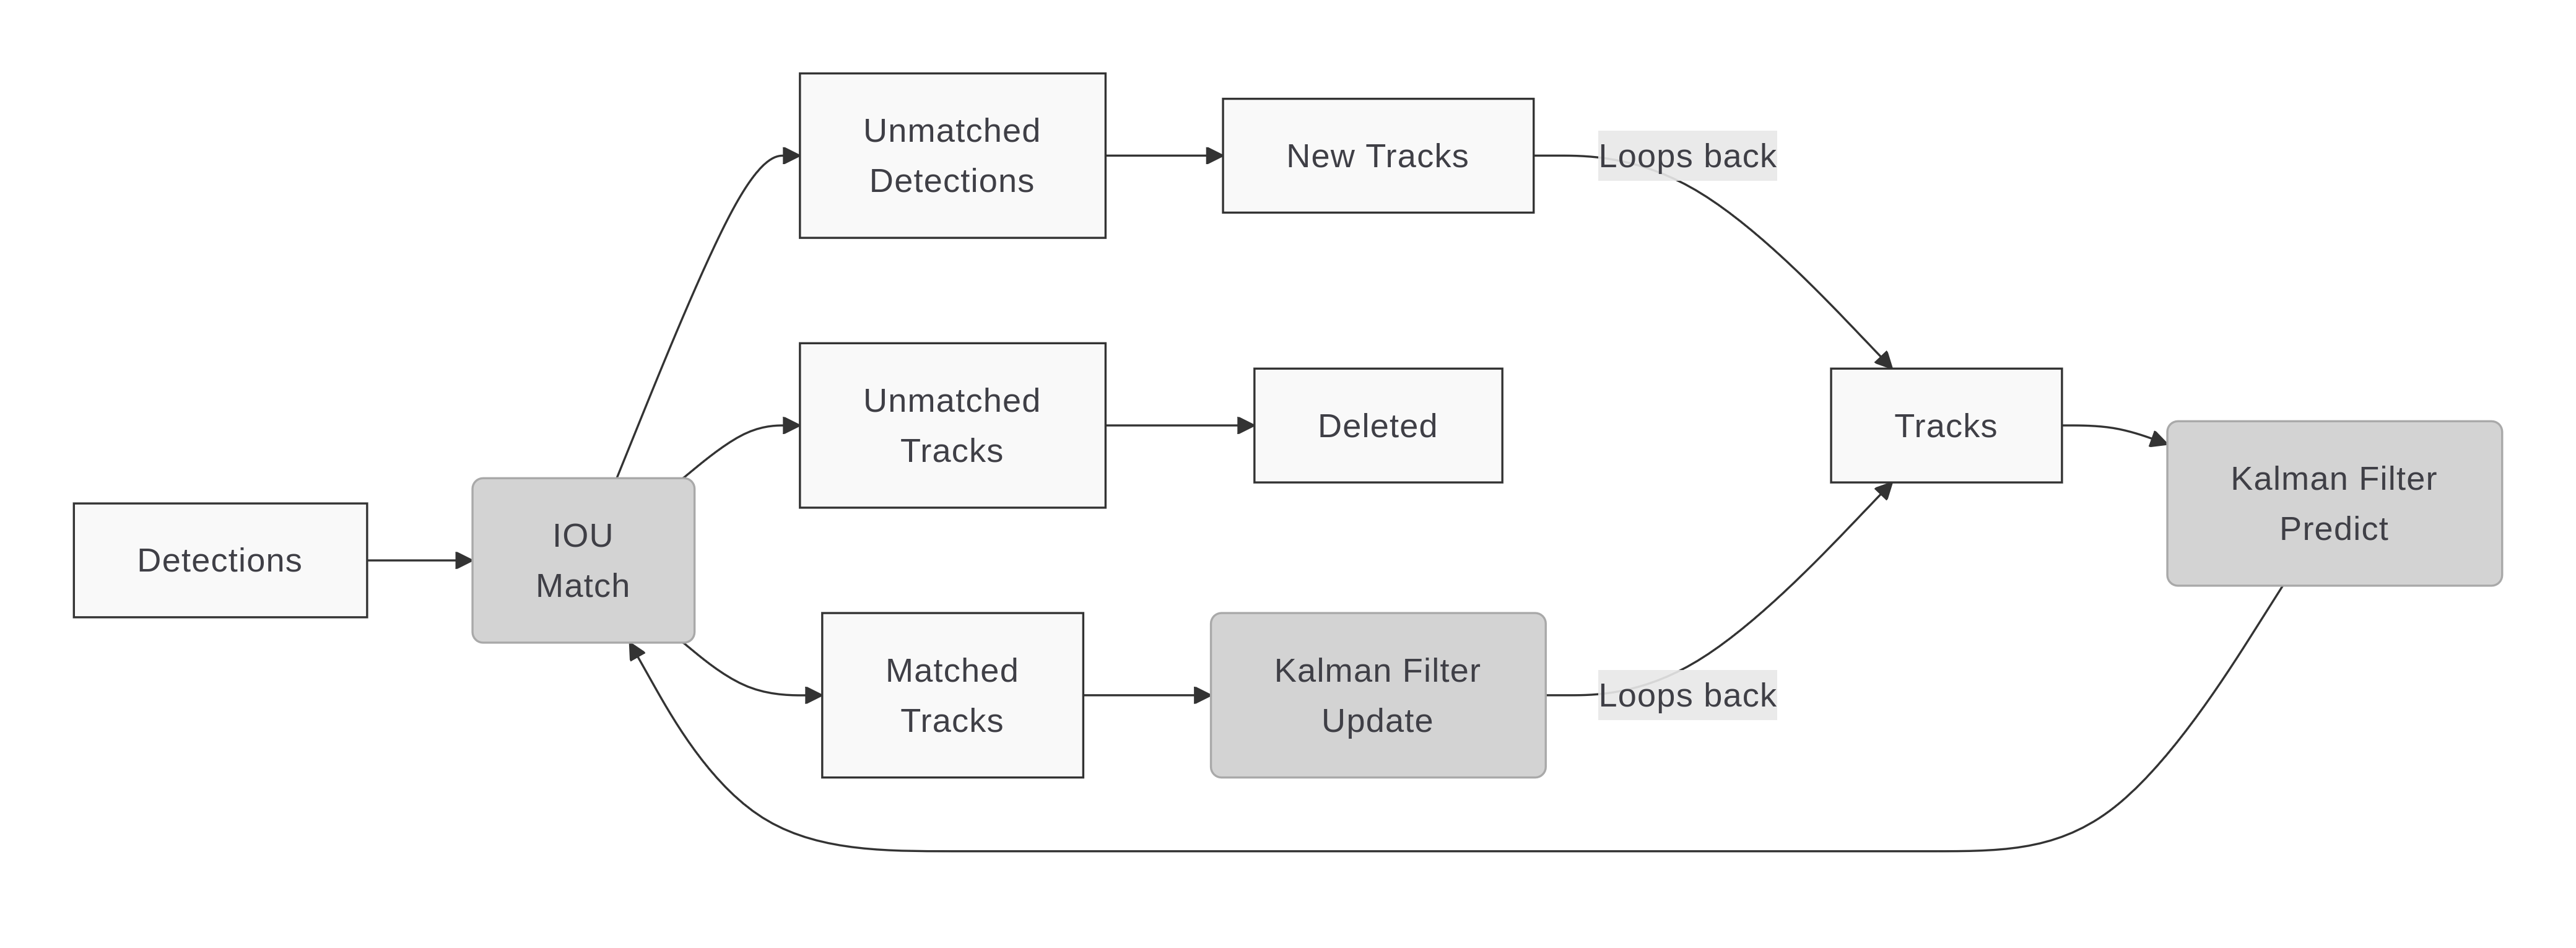
\includegraphics[width=1.0\linewidth]{sort.png}
    \caption{The flowchart for SORT}
    \label{fig:SORT}
\end{figure}
\subsection{Deep SORT}
SORT is a highly efficient algorithm for multiple object tracking. It operates within an eight-dimensional state space $x = (u,v,\gamma,h,\dot{x},\dot{y},\dot{\gamma},\dot{h})$, where $(u, v)$ represents the bounding box center, $\gamma$ is the aspect ratio, and $h$ is the height. 

While original SORT performs well using Kalman filtering and Intersection over Union (IoU) matching, it frequently struggles with object occlusions, \textbf{leading to a high number of identity switches}. When an object is occluded, the uncertainty in state estimation increases, causing purely spatial association to become inaccurate. \textbf{\cite{deepsort}Deep SORT solves this by integrating visual appearance features, reducing identity switches by 45\% while maintaining real-time speeds.}

To improve tracking stability, Deep SORT utilizes a Convolutional Neural Network (CNN) pre-trained on a large-scale person re-identification dataset. 

\begin{itemize}
    \item \textbf{Offline Pre-training:} The network learns deep appearance descriptors, denoted as $r_j$ (where $\|r_j\| = 1$), for bounding boxes. This moves the heavy computational burden offline.
    \item \textbf{Online Efficiency:} During real-time execution, the system only needs to perform fast nearest-neighbor queries in the visual appearance space to establish track associations.
\end{itemize}

When calculating the assignment cost between predicted tracks and new detections, Deep SORT elegantly balances spatial motion and visual characteristics by combining two distinct metrics:

\begin{itemize}
    \item \textbf{Motion Metric (Mahalanobis Distance):} 
    Evaluates the short-term motion match. It measures how many standard deviations a detection $d_j$ is from the Kalman filter's predicted mean track location $y_i$.
    \begin{equation}
        d^{(1)}(i,j) = (d_j - y_i)^T S_i^{-1} (d_j - y_i)
    \end{equation}
    
    \item \textbf{Appearance Metric (Cosine Distance):} 
    Crucial for recovering identities after long-term occlusions. It compares the CNN-generated descriptor $r_j$ against a gallery $\mathcal{R}_i$ of the last 100 associated descriptors for track $i$.
    \begin{equation}
        d^{(2)}(i,j) = \min \{1 - r_j^T r_k^{(i)} \mid r_k^{(i)} \in \mathcal{R}_i\}
    \end{equation}
\end{itemize}

These metrics are fused into a single weighted cost matrix:
\begin{equation}
    c_{i,j} = \lambda d^{(1)}(i,j) + (1-\lambda)d^{(2)}(i,j)
\end{equation}
An association is only considered admissible if it falls within the 95\% confidence interval gating region of both metrics, denoted by the indicator variable $b_{i,j} = \prod_{m=1}^{2} b_{i,j}^{(m)}$.

A major algorithmic contribution of Deep SORT is the Matching Cascade, designed to handle the uncertainty caused by prolonged occlusions. When an object is occluded, the Kalman filter's probability distribution spreads out. Counterintuitively, the Mahalanobis distance favors this larger uncertainty, which can cause track fragmentation when multiple tracks compete for the same detection. 

To prevent this, \textbf{the Matching Cascade (Algorithm 2) replaces a single global assignment with a series of smaller subproblems ordered by track age $a_i$.} (The age is defined as the number of frames that a track was not matched to an object, it's reset to 0 if it's matched.) \textbf{It prioritizes tracks that have been matched more recently, ensuring active objects are associated first.}

\begin{algorithm}[H]
\caption{Matching Cascade}
\begin{algorithmic}[1]
\Require Track indices $\mathcal{T} = \{1, \dots, N\}$, Detection indices $\mathcal{D} = \{1, \dots, M\}$, Maximum age $A_{max}$
\State Compute cost matrix $C = [c_{i,j}]$ using Equation 3
\State Compute gate matrix $B = [b_{i,j}]$ to isolate admissible associations
\State Initialize set of matches $\mathcal{M} \gets \emptyset$
\State Initialize set of unmatched detections $\mathcal{U} \gets \mathcal{D}$
\For{$n = 1$ \textbf{to} $A_{max}$}
    \State Select tracks by age $\mathcal{T}_n \gets \{i \in \mathcal{T} \mid a_i = n\}$
    \State $[x_{i,j}] \gets \text{min\_cost\_matching}(C, \mathcal{T}_n, \mathcal{U})$
    \State $\mathcal{M} \gets \mathcal{M} \cup \{(i, j) \mid b_{i,j} \cdot x_{i,j} > 0\}$
    \State $\mathcal{U} \gets \mathcal{U} \setminus \{j \mid \sum_i b_{i,j} \cdot x_{i,j} > 0\}$
\EndFor
\State \Return $\mathcal{M}, \mathcal{U}$
\end{algorithmic}
\end{algorithm}

After the cascade matching process is complete, the system performs one final association stage. It applies the standard IoU association from the original SORT algorithm to any remaining unmatched or unconfirmed tracks of age $n=1$. This acts as a robust safety net to account for sudden appearance changes or partial occlusions caused by static scene geometry.
\subsection{Strong SORT}
\subsubsection{Upgrading DeepSORT to \cite{strongsort}StrongSORT}
To build a highly accurate online tracker, StrongSORT incorporates several advanced modules into the original DeepSORT architecture:

\begin{itemize}
    \item \textbf{BoT Feature Extractor:} StrongSORT replaces the simple CNN with a more powerful appearance feature extractor BoT (Bag of Tricks), enabling the extraction of highly discriminative features.
    
    \item \textbf{Exponential Moving Average (EMA):} Instead of maintaining a raw feature bank of the last 100 frames, StrongSORT updates the appearance state $e_i^t$ for the $i$-th tracklet at frame $t$ using an EMA mechanism. This leverages inter-frame feature changes to depress detection noise:
    \begin{equation}
        e_i^t = \alpha e_i^{t-1} + (1-\alpha)f_i^t
    \end{equation}
    where $f_i^t$ is the appearance embedding of the current matched detection, and $\alpha = 0.9$ is the momentum term.
    
    \item \textbf{NSA Kalman Filter:} Standard linear Kalman filters assume constant observation noise. NSA Kalman adaptively calculates the noise covariance $\tilde{R}_k$ based on the detection confidence score $c_k$:
    \begin{equation}
        \tilde{R}_k = (1 - c_k)R_k
    \end{equation}
    This ensures that lower-quality detections have less influence on the state update.
    
    \item \textbf{Combined Motion Cost \& Vanilla Matching:} StrongSORT abandons the matching cascade in favor of a vanilla global linear assignment. The assignment cost matrix $C$ combines the appearance cost $A_a$ and motion cost $A_m$:
    \begin{equation}
        C = \lambda A_a + (1-\lambda)A_m
    \end{equation}
    where $\lambda = 0.98$ heavily weights the appearance features while still respecting spatial boundaries.
\end{itemize}

\subsubsection{Post-Processing: StrongSORT++}
To address the inherent MOT challenges of ``missing associations'' and ``missing detections,'' two lightweight algorithms are introduced. When combined with StrongSORT, the resulting model is StrongSORT++.

\noindent\textbf{Appearance-Free Link (AFLink)}
Missing associations occur when tracking is interrupted, breaking a trajectory into short tracklets. AFLink is an offline global linking model that predicts the connectivity between two tracklets relying exclusively on spatiotemporal information, represented as $T_* = \{f_k^*, x_k^*, y_k^*\}_{k=k^*}^{k^*+N-1}$. By using a CNN to process frame numbers and coordinates while completely ignoring appearance features, it avoids occlusion vulnerabilities.

\begin{algorithm}[H]
\caption{AFLink Global Association Strategy}
\begin{algorithmic}[1]
\Require Set of all tracklets $\mathcal{T}$, Temporal threshold $\Delta t_{max}$, Spatial threshold $\Delta s_{max}$, Score threshold $\tau$
\State Initialize valid pairs candidate set $\mathcal{P} \gets \emptyset$
\For{each pair $(T_i, T_j)$ in $\mathcal{T}$}
    \If{time\_gap$(T_i, T_j) < \Delta t_{max}$ \textbf{and} spatial\_dist$(T_i, T_j) < \Delta s_{max}$}
        \State $\text{score}_{i,j} \gets \text{AFLink\_CNN}(T_i, T_j)$
        \If{$\text{score}_{i,j} \ge \tau$}
            \State $\mathcal{P} \gets \mathcal{P} \cup \{(T_i, T_j, \text{score}_{i,j})\}$
        \EndIf
    \EndIf
\EndFor
\State $\mathcal{M} \gets \text{GlobalLinearAssignment}(\mathcal{P})$ \Comment{Solve via Hungarian Algorithm}
\State \Return $\mathcal{M}$
\end{algorithmic}
\end{algorithm}

\noindent\textbf{Gaussian-Smoothed Interpolation (GSI)}
Missing detections are traditionally handled with linear interpolation, which ignores motion dynamics. GSI uses Gaussian Process Regression (GPR) to model nonlinear motion, acting as a detection noise filter. The motion is formulated as:
\begin{equation}
    p_t = f^{(i)}(t) + \epsilon, \quad \text{where} \quad \epsilon \sim \mathcal{N}(0, \sigma^2)
\end{equation}
Assuming $f^{(i)}$ follows a Gaussian process $f^{(i)} \sim \mathcal{GP}(0, k(\cdot, \cdot))$ with a radial basis function (RBF) kernel $k(x, x') = \exp(-\frac{\|x-x'\|^2}{2\lambda^2})$, GSI smooths the entire trajectory. The smoothness factor $\lambda$ adaptively scales with the length of the tracklet, producing highly accurate and stable localizations.
\subsection{ByteTrack}
Most of the previously introduced MOT algorithms filter out bounding boxes with low confidence scores, ignoring them as background noise.

The core innovation of \cite{bytetrack}ByteTrack lies in its two-stage matching process that treats low-score detection boxes as a bridge to recover difficult objects and filter out background noise. The strategy proceeds as follows:

\begin{itemize}
    \item \textbf{Detection Separation:} For each frame, the detector yields a set of bounding boxes. These are divided into two sets based on a threshold $\tau$: high-score detections $\mathcal{D}_{high}$ and low-score detections $\mathcal{D}_{low}$.
    \item \textbf{First Association (High-Score):} The algorithm first matches the high-score detection boxes $\mathcal{D}_{high}$ to the predicted existing tracklets $\mathcal{T}$. This step uses a similarity metric (Similarity\#1), which can be Intersection over Union (IoU) or a Re-ID feature distance.
    \item \textbf{Second Association (Low-Score):} Some tracklets remain unmatched after the first stage, often because the object was occluded or blurred, dropping its detection score below $\tau$. BYTE then performs a second association between the unmatched tracklets $\mathcal{T}_{remain}$ and the low-score detections $\mathcal{D}_{low}$. 
    \item \textbf{IoU-Only Metric:} It is crucial that the second association relies \textit{only} on spatial IoU (Similarity\#2) rather than appearance features. Low-score boxes usually contain severe occlusion or motion blur, making appearance features highly unreliable. Unmatched low-score detections are subsequently discarded as background.
\end{itemize}


By equipping the highly efficient BYTE association method with the high-performance YOLOX object detector, the authors propose the strong tracking framework known as ByteTrack. Because it operates without computationally heavy appearance extractors in its standard form, it achieves state-of-the-art accuracy while running at high frame rates (e.g., 30 FPS).

The tracking pipeline is summarized in the following algorithm:

\begin{algorithm}[H]
\caption{BYTE Association Strategy}
\begin{algorithmic}[1]
\Require Video sequence $V$, Object detector $Det$, Detection score threshold $\tau$
\State Initialize tracks $\mathcal{T} \gets \emptyset$
\For{each frame $f_k$ in $V$}
    \State $\mathcal{D}_k \gets Det(f_k)$
    \State $\mathcal{D}_{high} \gets \emptyset$, $\mathcal{D}_{low} \gets \emptyset$
    \For{each $d$ in $\mathcal{D}_k$}
        \If{$d.score > \tau$}
            \State $\mathcal{D}_{high} \gets \mathcal{D}_{high} \cup \{d\}$
        \Else
            \State $\mathcal{D}_{low} \gets \mathcal{D}_{low} \cup \{d\}$
        \EndIf
    \EndFor
    
    \For{each track $t$ in $\mathcal{T}$}
        \State $t_{pred} \gets \text{KalmanFilter}(t)$ \Comment{Predict new locations}
    \EndFor
    
    \State \textbf{/* First Association */}
    \State Associate $\mathcal{T}$ and $\mathcal{D}_{high}$ using Similarity\#1
    \State $\mathcal{D}_{remain} \gets$ remaining unmatched detections from $\mathcal{D}_{high}$
    \State $\mathcal{T}_{remain} \gets$ remaining unmatched tracks from $\mathcal{T}$
    
    \State \textbf{/* Second Association */}
    \State Associate $\mathcal{T}_{remain}$ and $\mathcal{D}_{low}$ using Similarity\#2 (IoU only)
    \State $\mathcal{T}_{re-remain} \gets$ remaining unmatched tracks from $\mathcal{T}_{remain}$
    
    \State Mark $\mathcal{T}_{re-remain}$ as lost/deleted
    \For{each $d$ in $\mathcal{D}_{remain}$}
        \State $\mathcal{T} \gets \mathcal{T} \cup \{d\}$ \Comment{Initialize new tracks}
    \EndFor
\EndFor
\State \Return $\mathcal{T}$
\end{algorithmic}
\end{algorithm}















\subsection{OC-SORT}
MOT methods such as SORT, DeepSORT and StrongSORT all build upon a Kalman filter (KF) with a linear motion assumption. While DeepSORT and StrongSORT augment SORT with deep re-identification features to reduce identity switches, they inherit its fundamental motion model unchanged. 

All three follow an \textit{estimation-centric} design: when no detection is available during occlusion, the KF performs a dummy update $\hat{\mathbf{x}}_{t|t} = \hat{\mathbf{x}}_{t|t-1}$, blindly trusting the prior estimate rather than leveraging any observation signal. This causes positional noise to grow quadratically as $\delta_{u_{t+T}} \sim \mathcal{N}(0, 2T^2\sigma_u^2)$, easily reaching the scale of the object within 10 occluded frames. 

OC-SORT\cite{ocsort} directly addresses the structural disadvantages above by rethinking the role of observations in the tracking pipeline. Rather than relying solely on KF state estimates, it proposes an \textbf{observation-centric} design that uses detector outputs more aggressively, both for association and for correcting accumulated KF error after occlusion. The method remains purely motion-based, online, and runs at $700+$ FPS on a single CPU.

There are two key designs in OC-SORT:
\begin{itemize}
    \item Observation-Centric Re-Update (ORU): Uses observations to correct the accumulated error during the occlusion period.
    \item Observation-Centric Momentum (OCM): Introduces a "direction consistency" term into the association stage, but instead of relying on state estimates, it relies on real observations.
\end{itemize}


\subsubsection{Observation-Centric Re-Update (ORU)}

One of the core innovation of OC-SORT is the ORU module, which activates whenever a lost track is re-associated with a detection after $T$ occluded frames. Instead of accepting the degraded KF state at re-association time, ORU \textit{backtracks} the KF along a \textbf{virtual trajectory} interpolated between the last observed state $\mathbf{z}_{t_1}$ (before occlusion) and the re-associating observation $\mathbf{z}_{t_2}$. Under a constant-velocity assumption, the virtual trajectory is:
\begin{equation}
    \tilde{\mathbf{z}}_t = \mathbf{z}_{t_1} + \frac{t - t_1}{t_2 - t_1}(\mathbf{z}_{t_2} - \mathbf{z}_{t_1}),
    \quad t_1 < t < t_2.
\end{equation}
The Kalman filter is then re-run along this trajectory using a \textit{re-update} stage:
\begin{equation}
    \text{re-update}
    \begin{cases}
        \mathbf{K}_t = \mathbf{P}_{t|t-1}\mathbf{H}_t^\top
                       \left(\mathbf{H}_t \mathbf{P}_{t|t-1}\mathbf{H}_t^\top + \mathbf{R}_t\right)^{-1},\\[4pt]
        \hat{\mathbf{x}}_{t|t} = \hat{\mathbf{x}}_{t|t-1}
                       + \mathbf{K}_t\!\left(\tilde{\mathbf{z}}_t - \mathbf{H}_t\hat{\mathbf{x}}_{t|t-1}\right),\\[4pt]
        \mathbf{P}_{t|t} = (\mathbf{I} - \mathbf{K}_t\mathbf{H}_t)\,\mathbf{P}_{t|t-1}.
    \end{cases}
\end{equation}
This design replaces the dummy updates accumulated during occlusion with observation-grounded corrections.

\subsubsection{Observation-Centric Momentum (OCM)}

To exploit the linear motion assumption more reliably, OC-SORT incorporates a velocity direction consistency term into the association cost. 

The key insight is that a direction estimated from two \textbf{observations} separated by $\Delta t$ steps is far less noisy than one computed from KF estimates, because observations carry i.i.d.\ noise whereas KF estimates accumulate error over time.

Given $N$ existing tracks and $M$ new detections, the association cost matrix is:
\begin{equation}
    C(\hat{\mathbf{X}}, \mathbf{Z}) = C_{\text{IoU}}(\hat{\mathbf{X}}, \mathbf{Z})
                                    + \lambda\, C_v(\mathcal{Z}, \mathbf{Z}),
\end{equation}
where $C_{\text{IoU}}$ is the standard negative pairwise IoU cost and $C_v$ penalizes inconsistency between the historical motion direction of a track and the direction implied by linking the track's last observation to a candidate new detection:
\begin{equation}
    \theta = \arctan\!\left(\frac{v_1 - v_2}{u_1 - u_2}\right),
    \quad
    \Delta\theta = |\theta^{\text{track}} - \theta^{\text{intention}}|.
\end{equation}
The weighting is set to $\lambda = 0.2$ and the direction is computed using observations $\Delta t = 3$ steps apart, balancing noise reduction against the validity of the linear approximation.

As a lightweight complement to ORU and OCM, OC-SORT includes an heuristic technique called OCR (Observation-Centric Recovery).

After the primary association stage, unmatched tracks attempt a second association using their \textbf{last observed bounding box} (rather than the KF estimate) against remaining unmatched detections.\textbf{ This handles short stoppages and brief occlusions without invoking the full ORU mechanism.}
\begin{figure}[H]
    \centering
    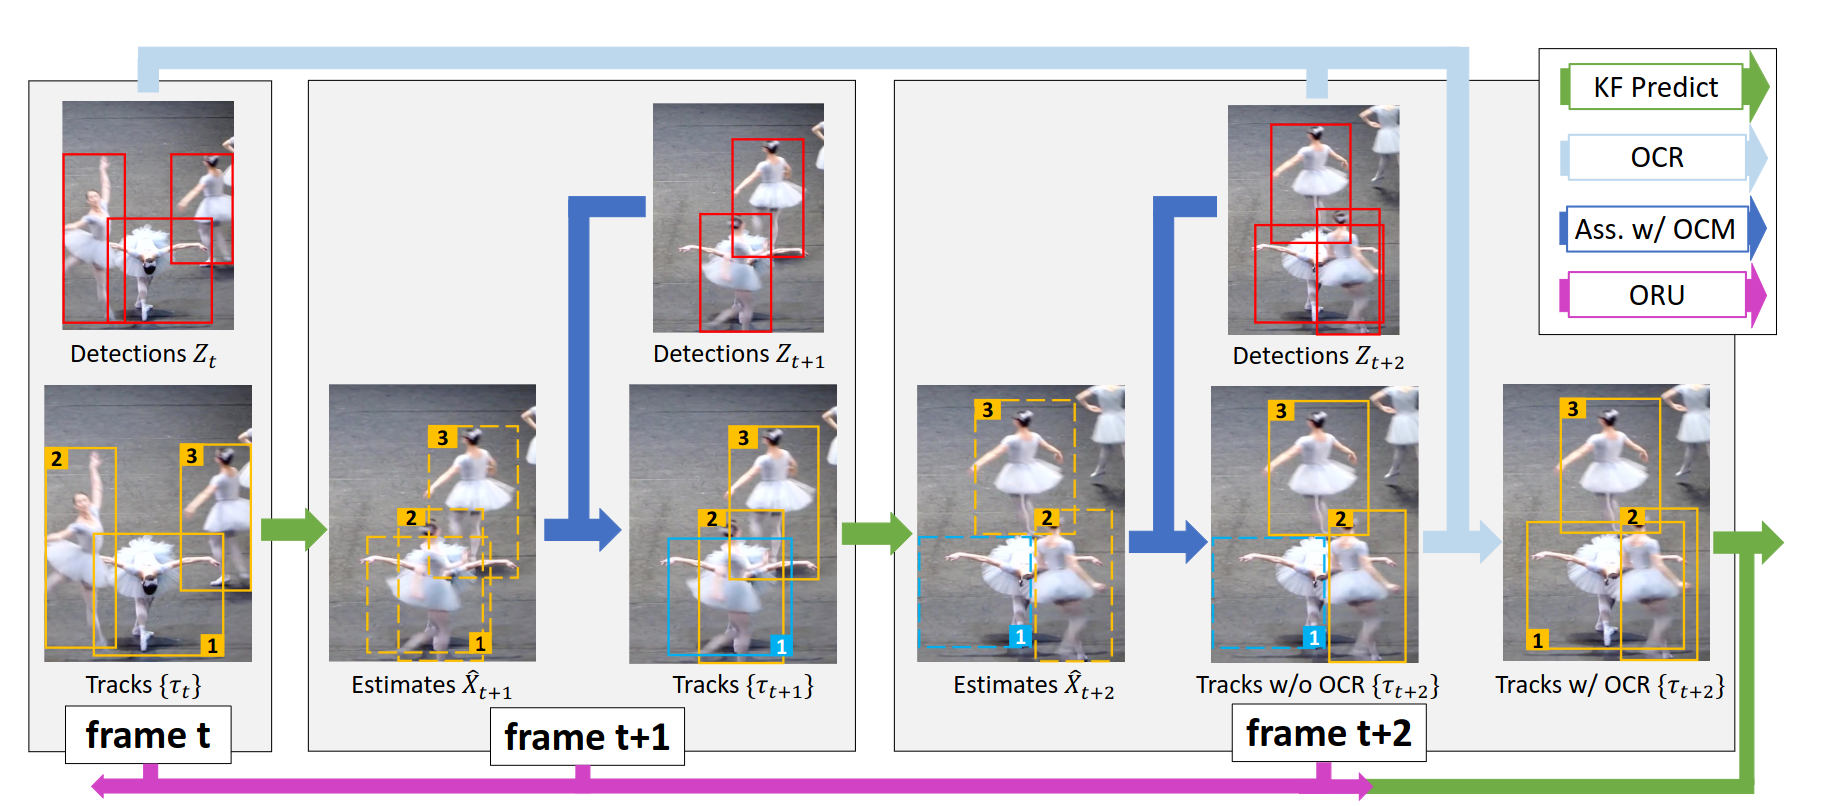
\includegraphics[width=\linewidth]{ocsort_pipeline.png}
    \caption{}
    \label{fig:ocsort}
\end{figure}
The overall process of OC-SORT can be demonstrated using the above figure \ref{fig:ocsort}. In the OC-SORT pipeline, detections are shown as red boxes, active tracks as orange boxes, untracked targets as blue boxes, and KF state estimates as dashed boxes. 

During the association stage, OCM incorporates a velocity direction consistency cost to improve matching. Target 1 becomes lost at frame $t+1$ due to occlusion, but is successfully recovered at frame $t+2$ by OCR, which re-associates it using its last known observation from frame $t$. This re-association then triggers ORU, which backtracks and corrects the KF parameters over the interval from $t$ to $t+2$.


\section{Comparison}
\subsection{Evaluation metrics}
The most commonly used metrics is \textbf{MOTA (Multiple Object Tracking Accuracy)}, which measures overall tracking accuracy by combining False Positives (FP), False Negatives (FN), and Identity Switches (IDSW), independent of localization precision. The formula is:
$$\displaystyle 1 - \frac{\sum_t (FN_t + FP_t + IDSW_t)}{\sum_t GT_t}$$

A larger MOTA often implies a higher level of model precision. To improve readability, we will also briefly introduce some metrics for evaluating MOT algorithms:
\begin{itemize}    
    \item \textbf{MOTP (Multiple Object Tracking Precision):} Measures the average localization precision (bounding box overlap or distance) of matched targets, which is calculated by:
    $$\displaystyle \frac{\sum_{t,i} d_{t,i}}{\sum_t c_t}$$
    
    \item \textbf{IDF1 (Identification F1-Score):} Harmonic mean of ID Precision and Recall; evaluates the tracker's ability to maintain consistent identities, which is calculated by:
    $$\displaystyle \frac{2 \times IDTP}{2 \times IDTP + IDFP + IDFN}$$
    
    \item \textbf{MT (Mostly Tracked):} Percentage of ground-truth (GT) trajectories successfully tracked for at least $80\%$ of their lifespan, which is calculated by:
    $$\displaystyle \frac{N_{\text{tracked } \ge 80\%}}{N_{\text{total GT}}}$$
    
    \item \textbf{ML (Mostly Lost):} Percentage of ground-truth (GT) trajectories successfully tracked for less than $20\%$ of their lifespan, which is calculated by:
    $$ML=\displaystyle \frac{N_{\text{tracked } < 20\%}}{N_{\text{total GT}}}$$
    
    \item \textbf{Frag (Fragmentation):} Total number of times a ground-truth trajectory is interrupted (tracking lost, but later resumes), which is calculated by:
    $$Frag=\displaystyle \sum (\text{Track Interruptions})$$
\end{itemize}
\subsection{Experiments}
In the papers I surveyed, most study used MOT challenge dataset to test the performance of their proposed approach.

In this survey I use the results tested on MOT17 to compare these algorithms. MOT17 uses the exact same video sequences as MOT16 but with more precise ground-truth annotations. A key feature of MOT17 is that it provides three different sets of public object detections (DPM, Faster R-CNN, and SDP) for each video. This allows researchers to evaluate how well their tracking algorithms perform regardless of the underlying detector's quality.
\begin{table}[H]
    \centering
    \resizebox{\columnwidth}{!}{
    \begin{tabular}{lccccc}
        \hline
        \textbf{Algorithm} & \textbf{MOTA} $\uparrow$ & \textbf{IDF1} $\uparrow$ & \textbf{HOTA} $\uparrow$ & \textbf{IDs} $\downarrow$ & \textbf{FPS} $\uparrow$ \\
        \hline
        SORT \cite{strongsort} & 43.1 & 39.8 & 34.0 & 4,852 & 143.3 \\
        DeepSORT \cite{strongsort} & 61.2 & 74.5 & 61.2 & 1,821 & 13.8 \\
        StrongSORT \cite{strongsort} & 78.3 & 78.5 & 63.5 & 1,446 & 7.5 \\
        ByteTrack \cite{bytetrack} & 80.3 & 77.3 & 63.1 & 2,196 & 29.6 \\
        OC-SORT \cite{ocsort} & 78.0 & 77.5 & 63.2 & 1,950 & 700+* \\
        \hline
    \end{tabular}
    }
    \caption{Performance comparison on the MOT17 test set (Private Detections). *OC-SORT FPS is evaluated purely on the association step.}
    \label{tab:mot_comparison}
\end{table}
The results highlight a clear evolution in MOT algorithms. The baseline SORT is extremely fast (143.3 FPS) but struggles with occlusions, resulting in lower accuracy and frequent identity switches. 

DeepSORT and StrongSORT solve these identity issues and boost accuracy (up to 78.3 MOTA) by adding deep appearance features, but this computational overhead drops their speed to under 15 FPS.

Some SOTA methods like ByteTrack and OC-SORT achieve excellent accuracy (up to 80.3 MOTA) while restoring real-time speeds by replacing heavy appearance embeddings with advanced spatial and observation-centric tracking strategies.
\section{Conclusion}
In conclusion, this survey highlights the evolution of MOT algorithms in balancing speed and accuracy. 

While the SORT baseline is exceptionally fast, it struggles heavily with occlusions.

DeepSORT and StrongSORT resolve these identity switches using deep appearance features, but their computational overhead prevents real-time application.

State-of-the-art models like ByteTrack and OC-SORT solve this dilemma. \textbf{By relying on advanced spatial association and raw observation corrections instead of heavy visual features, they achieve both top-tier accuracy and the real-time speeds crucial for autonomous driving.}
\newpage
\bibliographystyle{plain}
\bibliography{main}
\end{document}
